% !TEX root = ./main.tex
%%%%%%%%%%%%%%%%%%%%%%%%%%%%%%%%%%%%%%%%%%%%%%%%%%%%%%%%%%%%%%%%%%%%%%%%%%%%%%%%%%%%%%%%%%
% Dans cette section, indiquez et décrivez tous les Invariants nécessaires.              %
%                                                                                        %
% Pour chaque SP nécessitant un Invariant (une sous-section/SP):                         %
% - Donnez l'Invariant Graphique                                                         %
% - Donnez l'Invariant Formel correspondant à l'Invariant Graphique                      %
% Pensez à utiliser les notations définies précédemment.                                 %
%%%%%%%%%%%%%%%%%%%%%%%%%%%%%%%%%%%%%%%%%%%%%%%%%%%%%%%%%%%%%%%%%%%%%%%%%%%%%%%%%%%%%%%%%%
\section{Invariants}\label{invariants}
%%%%%%%%%%%%%%%%%%%%
\subsection{Explications}
La raison d'être de cette section est de définir les invariants nécessaires à la
construction du programme. Les invariants sont des propriétés qui doivent être
vérifiées à chaque étape de l'exécution du programme. Ils permettent de garantir
que le programme fonctionne correctement et produit les résultats attendus. Il y
a une règle qui est que chaque boucle nécessite un invriant. Nous aurons donc 2
invariants graphiques et 2 invariants formels

Nous allons donc définir les invariants graphiques. Le premier aura pour objectif
de définir la boucle de décrementation de $k$ et le seconde couvrira la boucle
qui compare les valeurs du tableau entre $T[i]$ et $T[N-k+i]$.

\subsection{SP1}
\subsubsection{Invariant Graphique}
Pour le premier invariant, nous allons définir la boucle de décrementation de $k
$. La valeur de $k$ est initialisée à $N - 1$ et elle est décrémentée jusqu'à ce
qu'elle atteigne 0. Attention, elle atteint zéro uniquement si lors du SP2 nous 
n'avons trouvé aucune correspondance dans le tableau.
\begin{figure}[h]
   \centering
   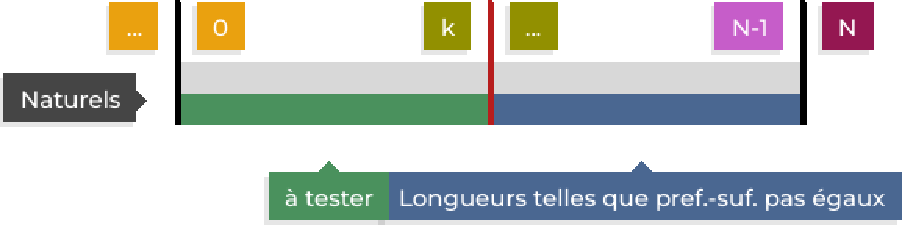
\includegraphics[width=0.5\textwidth]{sp1.pdf}
   \caption{Invariant graphique 1}
   \label{fig:invariant1}
\end{figure}

Le critère d'arrêt de la boucle est $k ==0$. Donc, le gardien de boucle sera
$k > 0$.

\subsubsection{Invariant Formel}

\begin{center}
   \fbox{
      \begin{minipage}{0.5\textwidth}
      \begin{center}
      $N = N_0$ \\
      $\wedge$ \\
      $ 0 \leq k \leq N - 1$ \\
      $\wedge$ \\
      k = max\_prefixe\_suffixe(*T, i ,N) \\
      \end{center}
      \end{minipage}
   }
\end{center}

\subsection{SP2}
\subsubsection{Invariant Graphique}
Pour le second invariant, nous allons définir la boucle de comparaison entre les
valeurs du tableau entre $T[i]$ et $T[N-k+i]$. La valeur de $i$ est initialisée 
à 0 et elle est incrémentée jusqu'à ce qu'elle atteigne $k$.

\begin{figure}[h]
   \centering
   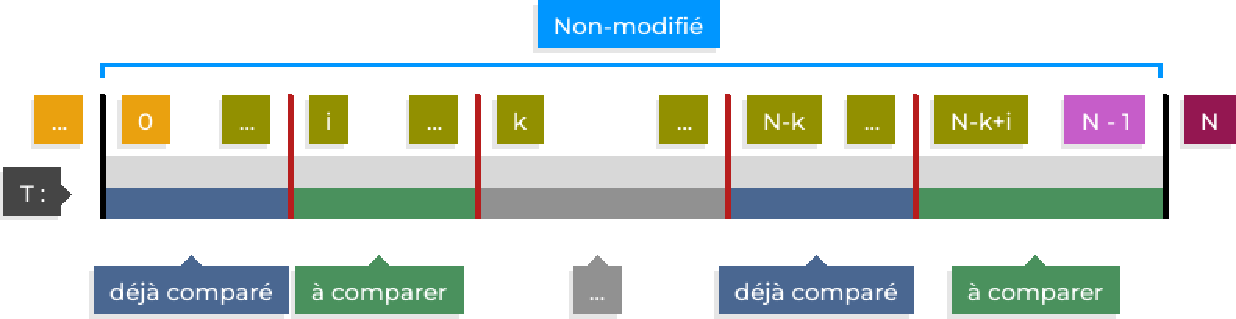
\includegraphics[width=0.5\textwidth]{sp2.pdf}
   \caption{Invariant graphique 2}
   \label{fig:invariant2}
\end{figure}

Le critère d'arrêt de la boucle est $i == k$. Donc, le gardien de boucle sera
$i < k$.
\subsubsection{Invariant Formel}

\begin{center}
   \fbox{
      \begin{minipage}{0.5\textwidth}
      \begin{center}
      $N = N_0 \wedge T = T_0$ \\
      $\wedge$ \\
      $ 0 \leq i < k$ $< N$\\
      $\wedge$ \\
      $T[i] = T[N-k+i]$ \\
      \end{center}
      \end{minipage}
   }
\end{center}